\section{Simplification of the Navier-Stokes equation}

\subsection{Simplification I: incompressible flows}
Incompressiblity is a very good approximation for most liquids, including water. In $\SI{1000}{m}$ depth the density of seawater is only $0.4\%$ larger than at the surface. For gas flows incompressiblity is also a good approximation as long as $|\vec{u}_\mathrm{gas}| \ll \mathrm{speed\ of\ sound}$. Compressibility becomes important when discussing e.g. sound waves.

Incompressibility means that the density of a fluid particle (moving along its pathline) remains constant.
\begin{align}
0 = \diff{\rho(\vec{r},t)}{t} &= \pdiff{\rho}{t}+\left(\vec{u}\cdot\vec{\nabla}\right)\rho\\
&= -\vec{\nabla}\left(\rho\vec{u}\right)+\left(\vec{u}\cdot\vec{\nabla}\right)\rho \\
&= -\left(\vec{u}\cdot\vec{\nabla}\right)\rho - \rho\left(\vec{\nabla}\cdot\vec{u}\right) + \left(\vec{u}\cdot\vec{\nabla}\right)\rho\\
&= -\rho\left(\vec{\nabla}\cdot\vec{u}\right)\\
&= -\rho\, \mathrm{div}\, \vec{u}
\end{align}
In the first line we used the material derivative. In the step to the second line we used continuity equation. For incompressibility the divergence must be zero:
\begin{equation}
\vec{\nabla}\cdot\vec{u} = 0
\end{equation}
Navier-Stokes equation for incompressible flows (3 equations):
\begin{equation}
\rho\left(\pdiff{\vec{u}}{t}+\left(\vec{u}\cdot\vec{\nabla}\right)\right)\vec{u} = f_\mathrm{ext}-\vec{\nabla}p+\mu\left(\vec{\nabla}\cdot\vec{\nabla}\right)\vec{u}
\end{equation}
\begin{framed}
Remark: It looks simple, but these nonlinear differential equations remain a formidable challenge to engineers, physicists and mathematicians.
\end{framed}
Fourth equation:
\begin{equation}
\vec{\nabla}\cdot\vec{u}=0.   
\end{equation}
Fifth equation: equation of state in the simplest form with constant density
\begin{equation}
p=p(\rho) \Rightarrow \rho=\rho_0=\mathrm{constant}.
\end{equation}


\subsection{Simplification II: incompressible, ideal, stationary, irrotational flows}
We use the incompressibility result:
\begin{equation}
\vec{\nabla}\cdot\vec{u} = 0
\end{equation}
Ideal means no friction. To eliminate friction forces we set $\mu=0$.

Euler equation:
\begin{equation}
\rho_0\left(\pdiff{\vec{u}}{t}+\left(\vec{u}\cdot\vec{\nabla}\right)\vec{u}\right) = \vec{f} _\mathrm{ext}-\vec{\nabla}p
\end{equation}
stationary:
\begin{align}
\vec{u}(\vec{r},t) &= \vec{u}(\vec{r})\\
\leadsto
\pdiff{\vec{u}}{t} &= 0
\end{align}
\begin{equation}
\rho_0\left(\vec{u}\cdot\vec{\nabla}\right)\vec{u} = \vec{f} _\mathrm{ext}-\vec{\nabla}p
\end{equation}
no external forces: $\vec{f} _\mathrm{ext}=0$
\begin{equation}
\rho_0\left(\vec{u}\cdot\vec{\nabla}\right)\vec{u} = -\vec{\nabla}p
\end{equation}
We now look at the convective term on the lefthand side (see the proof below):
\begin{align}
\left(\vec{u}\cdot\vec{\nabla}\right)\vec{u} &= \frac{1}{2}\vec{\nabla}\underbrace{\left(\vec{u}\cdot\vec{u}\right)}_{\vec{u}^2}- \vec{u}\times\left(\vec{\nabla}\times\vec{u}\right)\\
&\Downarrow\notag\\
\vec{\nabla}\left(\frac{\rho_0}{2}\vec{u}^2+p\right) &= \rho_0\vec{u}\times\left(\vec{\nabla}\times\vec{u}\right)
\end{align}

Assuming irrotational flow: $\vec{\nabla}\times\vec{u}=0$.
\begin{equation}
\vec{\nabla}\underbrace{\left(\frac{\rho_0}{2}\vec{u}^2+p\right)}_\mathrm{constant}=0
\end{equation}
Bernoulli's equation
\begin{align}
\frac{\rho_0}{2}\vec{u}^2+p &= \mathrm{constant}\\
\vec{\nabla}\cdot\vec{u} &= 0\\
\vec{\nabla}\times\vec{u} &= 0
\end{align}
Given all the assumptions, this set of equations is equivalent to the Navier-Stokes equation.

\begin{framed}
\textbf{Proof of}
\begin{equation}
\left(\vec{v}\cdot\vec{\nabla}\right)\vec{v}=\frac{1}{2}\vec{\nabla}\left(\vec{v}^2\right)-\vec{v}\times\left(\vec{\nabla}\times\vec{v}\right).
\end{equation}
First we look at the x-component of the left-hand side:
\begin{equation}
\left[\left(\vec{v}\cdot\vec{\nabla}\right)\vec{v}\right]_x = \left(v_x\partial_x+v_y\partial_y+v_z\partial_z\right)v_x
\end{equation}
Now we look at the rightmost term on the right-hand side:
\begin{equation}
\vec{\nabla}\times\vec{v} = \begin{vmatrix}
\vec{e}_x & \vec{e}_y & \vec{e}_z \\
\partial_x & \partial_y & \partial_z \\
v_x & v_y & v_z
\end{vmatrix} =
\left(\partial_yv_z-\partial_zv_y\right)\vec{e}_x +
\left(\partial_zv_x-\partial_xv_z\right)\vec{e}_y +
\left(\partial_xv_y-\partial_yv_x\right)\vec{e}_z
\end{equation}
Now we can show that the x-component of the right-hand side is equal to the x-component of the left-hand side:
\begin{align}
\begin{split}
\left[\frac{1}{2}\vec{\nabla}\left(\vec{v}^2\right)-\vec{v}\times\left(\vec{\nabla}\times\vec{v}\right)\right]_x &= \frac{1}{2}\partial_x\left(v_x^2+v_y^2+v_z^2\right)\\
&\hspace{3mm}- \begin{vmatrix}
\vec{e}_x & \vec{e}_y & \vec{e}_z \\
v_x & v_y & v_z \\
\partial_yv_z-\partial_zv_y & \partial_zv_x-\partial_xv_z & \partial_xv_y-\partial_yv_xv_x\left(\partial_xv_x\right)
\end{vmatrix}_x
\end{split}\\
\begin{split}
&= v_x\left(\partial_xv_x\right) + v_y\left(\partial_xv_y\right) + v_z\left(\partial_xv_z\right)\\
&\hspace{3mm}- v_y\left(\partial_xv_y-\partial_yv_x\right) + v_z\left(\partial_zv_x-\partial_xv_z\right)
\end{split}\\
&= v_x\left(\partial_xv_x\right)+v_y\left(\partial_yv_y\right)+v_z\left(\partial_zv_z\right)\\
&= \left[\left(\vec{v}\cdot\vec{\nabla}\right)\vec{v}\right]_x
\end{align}
\end{framed}


\subsection{Derivation of Bernoulli's equation}
The equation
\begin{equation}
\vec{\nabla}\left(\frac{\rho_0}{2}\vec{v}^2+p\right) = \rho_0\vec{v}\times\left(\vec{\nabla}\times\vec{v}\right)
\end{equation}
is (scalar) multiplied with $d\vec{s}\parallel\vec{v}$, where $d\vec{s}$ describes an increment of a specific streamline (here pathline since $\vec{v}(\vec{r},t) = \vec{v}(\vec{r})$).
\begin{equation}
d\vec{s}\cdot\left[\vec{v}\times\left(\vec{\nabla}\times\vec{v}\right)\right]=0
\end{equation}
Since $d\vec{s}\parallel\vec{v}$ it must be that $d\vec{s}\perp\vec{v}\times\left(\vec{\nabla}\times\vec{v}\right)$.

Subsequent path-integration along a streamline yields
\begin{align}
0 &\require \int_\text{streamline}\vec{\nabla}\underbrace{\left(\frac{\rho_0}{2}\vec{v}^2+p\right)}_W\cdot d\vec{s}\\
&= \int_\text{streamline} \begin{pmatrix}
\pdiff{W}{x}\\
\pdiff{W}{y}\\
\pdiff{W}{y}
\end{pmatrix}
\begin{pmatrix}
dx\\dy\\dz
\end{pmatrix}\\
&= \int_\text{streamline} \left(\pdiff{W}{x}dx+\pdiff{W}{y}dy+\pdiff{W}{z}dz\right)\\
&= \int_\text{streamline}dW = \int_\text{streamline} d\left(\frac{\rho_0}{2}\vec{v}^2+p\right)\\
&\Downarrow\notag\\
\frac{\rho_0}{2}\vec{v}^2+p&=\text{constant}\qquad\text{(along a streamline)}
\end{align}
For another streamline the constant might in principle be different. For examples like the velocity in the far-field regime is everywhere the same. The same holds true for the pressure. Then the "Bernoulli constant" has to be everywhere (far and nea-field) the same. From here we then also conclude that $\vec{\nabla}\times\vec{v}=0$ everywhere.

\subsection{Example: Why does an airplane fly?}
\begin{figure}[!h]
    \centering
    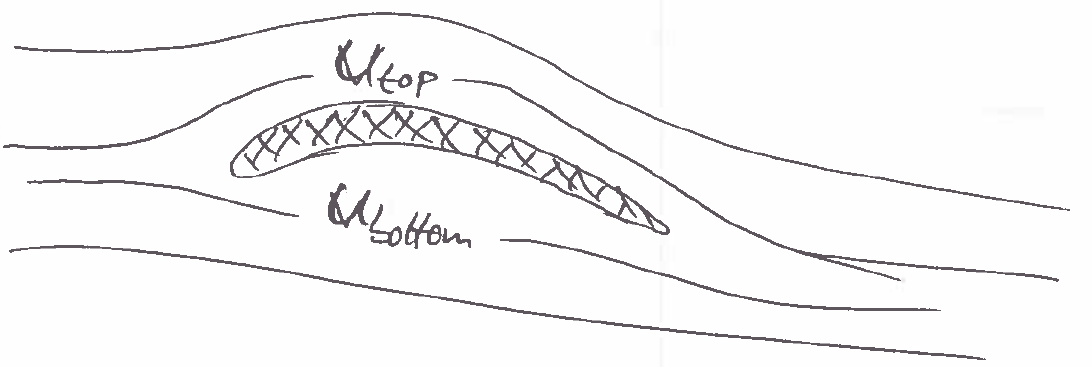
\includegraphics[width=.6\textwidth]{week2/airplane}
    \caption{The profile of the wing of an airplane.}
    \label{fig:airplane}
\end{figure}
The wind speed difference between the top and bottom of the wing creates a pressure difference:
\begin{align}
u_\mathrm{top} &> u_\mathrm{bottom}\\
\leadsto
p_\mathrm{top} &< p_\mathrm{bottom}.
\end{align}
This results in a lifting force.